\section{光滑目标与局部上界}
\label{sec:opt-smooth-local-bounds}

梯度只描述目标在当前点的一阶变化率，而算法每一步都要走出有限长度。一阶Taylor展开$f(\bm x+\bm p)\approx f(\bm x)+\langle\nabla f(\bm x),\bm p\rangle$在$\bm p\to\bm0$时成立，却没有说$\bm p$多大时误差可以忽略。本节回答局部导数信息怎样控制有限位移后的目标变化：先给梯度的变化速度规定上限，得到一阶模型的二次误差界；再把候选位移代入这个界，看出方向与步长各自承担什么作用。后面各节的求步规则和接受规则，都以这里的上界为共同依据。

本章反复使用一个二维例子：
\begin{equation}
\label{eq:opt-smooth-common-quadratic}
  f(\bm x)=\frac12\bigl(x_1^2+16x_2^2\bigr)=\frac12\bm x^\top\bm H\bm x,\qquad
  \bm H=\operatorname{diag}(1,16),\qquad
  \bm x^{(0)}=(2,2)^\top.
\end{equation}
它的最小点是原点，$f^\star=0$，初始目标值$f(\bm x^{(0)})=34$，梯度$\nabla f(\bm x)=\bm H\bm x=(x_1,16x_2)^\top$。两个坐标方向的曲率相差$16$倍，这个差别足以暴露本章讨论的大部分现象，而每一步又都能手算。

\subsection{梯度光滑性}
\label{sec:opt-smooth-lipschitz-gradient}

在共同例中，从某点沿$x_1$方向移动单位长度，梯度改变$(1,0)^\top$；沿$x_2$方向移动单位长度，梯度改变$(0,16)^\top$。同样长的位移，在陡的方向上使梯度改变得多，梯度变得越快，一阶近似失效得也越快。一般地，$\nabla f(\bm u)-\nabla f(\bm v)=\bm H(\bm u-\bm v)$，所以
\[
  \lVert\nabla f(\bm u)-\nabla f(\bm v)\rVert_2\leq\lVert\bm H\rVert_2\lVert\bm u-\bm v\rVert_2=16\lVert\bm u-\bm v\rVert_2,
\]
等号在$\bm u-\bm v$平行于$x_2$轴时取得。数字$16$是“每移动单位距离，梯度最多改变多少”的上限。对一般目标，我们要求同样的上限在关心的区域内统一存在。

\begin{definition}[梯度Lipschitz条件与$L$光滑]
\label{def:opt-smooth-l-smooth}
设$U\subseteq\mathbb R^d$，$f$在包含$U$的开集上可微，$L\geq0$。若对所有$\bm u,\bm v\in U$都有
\[
  \lVert\nabla f(\bm u)-\nabla f(\bm v)\rVert_2\leq L\lVert\bm u-\bm v\rVert_2,
\]
就说$\nabla f$在$U$上是$L$-Lipschitz的，也称$f$在$U$上\term{$L$光滑}（$L$-smooth）。$U=\mathbb R^d$时简称$f$为$L$光滑。
\end{definition}

这个条件比“可微”和“梯度连续”都强，三者需要分开。$f(x)=\tfrac23|x|^{3/2}$在$\mathbb R$上可微，导数$f'(x)=\operatorname{sign}(x)|x|^{1/2}$也连续，但$|f'(x)-f'(0)|/|x|=|x|^{-1/2}$在$x\to0$时无界，所以在包含原点的任何区间上都不存在光滑常数。$f(x)=x^4$无穷次可微，却因$f''(x)=12x^2$无界而不是全局$L$光滑；限制在$[-R,R]$上，由中值定理$|f'(u)-f'(v)|\leq12R^2|u-v|$，常数$12R^2$随区域变大。所以说一个目标“光滑”时，必须同时说明常数$L$和它成立的区域。

对二阶连续可微的目标，常数可以从Hessian读出。若$U$是凸开集且$\lVert\nabla^2f(\bm z)\rVert_2\leq L$对所有$\bm z\in U$成立，则对$\bm u,\bm v\in U$，沿线段积分得
\[
  \nabla f(\bm u)-\nabla f(\bm v)=\int_0^1\nabla^2f\bigl(\bm v+s(\bm u-\bm v)\bigr)(\bm u-\bm v)\,\mathrm ds,
\]
取范数即得$\lVert\nabla f(\bm u)-\nabla f(\bm v)\rVert_2\leq L\lVert\bm u-\bm v\rVert_2$。这里用到线段留在$U$中，这正是要求$U$为凸集的原因。对实对称矩阵，$\lVert\nabla^2f(\bm z)\rVert_2$等于其特征值绝对值的最大者；二次目标$\tfrac12\bm x^\top\bm H\bm x$的最小光滑常数就是$\bm H$的谱半径$\max_i|\lambda_i(\bm H)|$。实对称矩阵的正交谱分解与谱范数可参考\BookChapterRef{chap:linear-analysis}{卷一“谱和奇异值”章}；本章只用“二次型$\bm v^\top\bm H\bm v$介于最小与最大特征值乘$\lVert\bm v\rVert_2^2$之间”这一结论。

\paragraph{一阶模型的余项界}
有了梯度变化的上限，就能控制一阶模型与真实目标之差。

\begin{lemma}[下降引理]
\label{lem:opt-smooth-descent-lemma}
设$f$在凸集$U$上$L$光滑，$\bm x,\bm x+\bm p\in U$。则
\begin{equation}
\label{eq:opt-smooth-descent-lemma}
  \bigl|f(\bm x+\bm p)-f(\bm x)-\langle\nabla f(\bm x),\bm p\rangle\bigr|\leq\frac L2\lVert\bm p\rVert_2^2 .
\end{equation}
特别地，$f(\bm x+\bm p)\leq f(\bm x)+\langle\nabla f(\bm x),\bm p\rangle+\tfrac L2\lVert\bm p\rVert_2^2$。
\end{lemma}

\begin{proof}
令$\phi(s)=f(\bm x+s\bm p)$，$s\in[0,1]$。由于线段在$U$中，$\phi$可微且$\phi'(s)=\langle\nabla f(\bm x+s\bm p),\bm p\rangle$连续，于是
\[
  f(\bm x+\bm p)-f(\bm x)-\langle\nabla f(\bm x),\bm p\rangle
  =\int_0^1\bigl\langle\nabla f(\bm x+s\bm p)-\nabla f(\bm x),\bm p\bigr\rangle\,\mathrm ds .
\]
由Cauchy--Schwarz不等式和梯度Lipschitz条件，被积函数的绝对值不超过$\lVert\nabla f(\bm x+s\bm p)-\nabla f(\bm x)\rVert_2\lVert\bm p\rVert_2\leq Ls\lVert\bm p\rVert_2^2$，对$s$积分得$\tfrac L2\lVert\bm p\rVert_2^2$。
\end{proof}

引理的上半部分称为\term{下降引理}（descent lemma），因为后面会用它证明目标下降。它说：在当前点放一个开口向上、曲率为$L$的抛物面，这个抛物面在$\bm x$处与$f$相切，并且在整个$U$上盖住$f$；另一个开口向下的抛物面从下方托住$f$。图~\ref{fig:opt-smooth-upper-bound}画出了一维情形。$f(x)=\log(1+x^2)$的二阶导数$f''(x)=2(1-x^2)/(1+x^2)^2$取值在$[-1/4,2]$中，故$L=2$；在$x^{(0)}=1.5$处，两条抛物线夹住整条曲线。式~\eqref{eq:opt-smooth-descent-lemma}的证明只用到线段上的梯度，所以当$L$只在某个区域内成立时，候选点和连接它的线段都必须留在该区域中。

\begin{figure}[htbp]
  \centering
  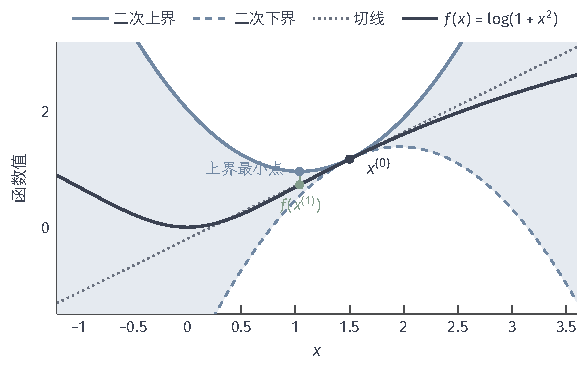
\includegraphics[width=99.5mm]{figures/03-optimization-evolution-and-signals/01-optimization/tikz/c3-quadratic-upper-bound/figure.pdf}
  \caption{一维目标$f(x)=\log(1+x^2)$在$x^{(0)}=1.5$处的二次上界与二次下界（$L=2$）。蓝色实线是$f(x^{(0)})+f'(x^{(0)})(x-x^{(0)})+(x-x^{(0)})^2$，虚线是把最后一项换成负号的下界，浅蓝区域夹住了黑色曲线。上界的最小点在$x^{(1)}=x^{(0)}-f'(x^{(0)})/L\approx1.038$，上界在该处的值约$0.966$；真实目标$f(x^{(1)})\approx0.732$（绿点）更低。}
  \label{fig:opt-smooth-upper-bound}
\end{figure}

\paragraph{共同例中的常数}
对式~\eqref{eq:opt-smooth-common-quadratic}，余项恰为$\tfrac12\bm p^\top\bm H\bm p=\tfrac12(p_1^2+16p_2^2)$，介于$\tfrac12\lVert\bm p\rVert_2^2$与$8\lVert\bm p\rVert_2^2$之间。$L=16$给出的上界只在$\bm p$平行于$x_2$轴时取等号；沿$x_1$方向，真实余项只有上界的$1/16$。这就是后面一切困难的来源：一个统一的常数必须照顾最陡的方向，因而对平坦方向过于保守。最小特征值$1$在这里对应第~\ref{chap:optimization}章的强凸常数$\mu$，它给出一阶模型误差的下界；本章记$\kappa=L/\mu$为条件数，共同例中$\kappa=16$。

\subsection{下降方向与模型上界}
\label{sec:opt-smooth-descent-direction}

有了上界，就可以把“选一个更新”拆成两个问题：沿哪个方向走，以及走多远。本小节先说明方向正确是什么意思，再说明为什么方向正确还不够。

\paragraph{下降方向}
在$\bm x$处沿方向$\bm d$的方向导数是$\langle\nabla f(\bm x),\bm d\rangle$。若它为负，就称$\bm d$为\term{下降方向}（descent direction）。由方向导数的定义，$f(\bm x+\eta\bm d)=f(\bm x)+\eta\langle\nabla f(\bm x),\bm d\rangle+o(\eta)$，所以存在$\bar\eta>0$，使$0<\eta<\bar\eta$时$f(\bm x+\eta\bm d)<f(\bm x)$。这个$\bar\eta$只是存在，定义没有告诉我们它有多大。负梯度$\bm d=-\nabla f(\bm x)$在非驻点处总是下降方向，因为$\langle\nabla f(\bm x),-\nabla f(\bm x)\rangle=-\lVert\nabla f(\bm x)\rVert_2^2<0$；任何与负梯度夹角小于直角的方向也是。

\paragraph{方向与步长的分工}
把位移$\eta\bm d$代入下降引理，记$\bm g=\nabla f(\bm x)$：
\begin{equation}
\label{eq:opt-smooth-direction-step}
  f(\bm x+\eta\bm d)\leq f(\bm x)+\eta\langle\bm g,\bm d\rangle+\frac{L\eta^2}{2}\lVert\bm d\rVert_2^2 .
\end{equation}
右边是$\eta$的二次函数。一次项由方向决定：只有$\langle\bm g,\bm d\rangle<0$时，小步长才能使右边低于$f(\bm x)$。二次项由步长决定：只有$0<\eta<2|\langle\bm g,\bm d\rangle|/(L\lVert\bm d\rVert_2^2)$时右边才严格低于$f(\bm x)$。在$\eta=|\langle\bm g,\bm d\rangle|/(L\lVert\bm d\rVert_2^2)$处右边最小，保证的下降量为
\[
  \frac{\langle\bm g,\bm d\rangle^2}{2L\lVert\bm d\rVert_2^2}=\frac{\lVert\bm g\rVert_2^2\cos^2\theta}{2L},
\]
其中$\theta$是$\bm d$与$-\bm g$的夹角。方向越偏离负梯度，能保证的下降越少；而方向再好，步长超出范围也可能上升。一维例子就能看到后者：$f(x)=8x^2$的$L=16$，在$x=1$处负梯度方向$d=-16$是下降方向，但取$\eta=0.2$得到$x=1-3.2=-2.2$，$f(-2.2)=38.72>8=f(1)$。方向没有错，错在步长越过了曲率允许的范围。

\paragraph{二次模型生成更新}
把方向和步长合在一起考虑，可以直接对整个位移$\bm p$最小化上界：
\[
  \min_{\bm p}\ f(\bm x)+\langle\bm g,\bm p\rangle+\frac L2\lVert\bm p\rVert_2^2 ,
\]
对$\bm p$求梯度并令其为零得$\bm p=-\bm g/L$，这正是步长$1/L$的梯度步，保证的下降量为$\lVert\bm g\rVert_2^2/(2L)$。图~\ref{fig:opt-smooth-upper-bound}中蓝点就是一维的这一步：在“碗盖”的最低处落脚，真实目标只会更低。

这个推理可以推广。对任意对称正定矩阵$\bm B$，考虑二次模型
\begin{equation}
\label{eq:opt-smooth-quadratic-model}
  m_{\bm B}(\bm p)=f(\bm x)+\langle\bm g,\bm p\rangle+\frac12\bm p^\top\bm B\bm p .
\end{equation}
它有唯一最小点$\bm p=-\bm B^{-1}\bm g$，且$\langle\bm g,\bm p\rangle=-\bm g^\top\bm B^{-1}\bm g<0$（$\bm g\neq\bm0$），所以无论$\bm B$怎样取，只要正定，模型步都是下降方向。取$\bm B=L\bm I$得到梯度下降；取固定的$\bm B=\bm P^{-1}$得到第~\ref{sec:opt-smooth-preconditioning}小节的预条件梯度法；取Hessian得到牛顿法；用观测到的梯度变化拼出$\bm B$得到拟牛顿法。只有当$\bm B$在相关区域内“盖得住”目标的曲率时，例如$\bm B=L\bm I$，模型最小点才自动保证原目标下降；其他选择下，模型只是近似，还需要线搜索、信赖域等接受规则用原目标核验。后续各方法的差别，就在于怎样构造$\bm B$、怎样求解模型，以及怎样决定接受与否。
